
\begin{table}[!ht]
\centering
\resizebox{\columnwidth}{!}{\begin{tabular}{|c|c|c|c|c|} 
\hline
Item & Number & Machine A & Machine B & Profit \\
\hline
Screw A & x & 4 minutes & 6 minutes & Rs 7 \\
\hline
Screw B & y & 6 minutes & 3 minutes & Rs 10 
\\
\hline
Max Available Time &  & 4hours  =240minutes & 4hours =240minutes &
\\
\hline
\end{tabular}}
\caption{Screw Requirements}
\label{opt/16/tab:table1}
\end{table}
Let the number of packages of screw  A be $x$ and the number of packages of screw B be $y$  such that 
\begin{align}
    x \geq 0 \\
    y \geq 0 
\end{align}
According to the question,
\begin{align}
    4x+6y &\leq 240 \\
 \implies 2x+3y &\leq 120
\end{align}
     and,
\begin{align}
    6x+3y &\leq 240 \\
 \implies 2x+y &\leq 80
\end{align}
$\therefore$ Our problem is
\begin{align}
        \max_{\vec{x}} Z &= \myvec{7 & 10}\vec{x}\\
        s.t. \quad 
        \myvec{2 & 3 \\ 2 & 1 }\vec{x} &\preceq \myvec{120\\80} 
\end{align}
Lagrangian function is given by
\begin{equation}
\begin{aligned}
    &L(\vec{x},\boldsymbol{\lambda}) \\ &= \myvec{7 & 10}\vec{x}+\lcbrak{\sbrak{\myvec{2 & 3}\vec{x}+120}} \\ &+ \sbrak{\myvec{2 & 1}\vec{x}+80} \\ &+ \sbrak{\myvec{-1 & 0}\vec{x}} +\rcbrak{\sbrak{\myvec{0 & -1}\vec{x}}}\boldsymbol{\lambda}
\end{aligned}
\end{equation}
where,
\begin{align}
    \boldsymbol{\lambda} &= \myvec{\lambda_1 \\ \lambda_2 \\ \lambda_3 \\ \lambda_4 \\ \lambda_5 \\ \lambda_6}
\end{align}
Now,
\begin{align}
    \nabla L(\vec{x},\boldsymbol{\lambda}) &= \myvec{7+ \myvec{2 & 3 & -1 & 0 }\boldsymbol{\lambda}\\ 10+\myvec{2 & 1 & 0 & -1}\boldsymbol{\lambda} \\ \myvec{2 & 3}\vec{x}+120 \\ \myvec{2 & 1}\vec{x}+80 \\ \myvec{-1 & 0}\vec{x} \\ \myvec{0 & -1}\vec{x}}
\end{align}
$\therefore$ Lagrangian matrix is given by
\begin{align}
    \myvec{0 & 0 & 2 & 3 & -1 & 0 \\ 0 & 0 & 2 & 1 & 0 & -1 \\ 2 & 3 & 0 & 0 & 0 & 0  \\ 2 & 1 & 0 & 0 & 0 & 0  \\ -1 & 0 & 0 & 0 & 0 & 0  \\ 0 & -1 & 0 & 0 & 0 & 0 }\myvec{\vec{x} \\ \boldsymbol{\lambda} } &= \myvec{-5 \\ -6 \\ 200 \\ 240 \\ 0 \\0 }
\end{align}
Considering $\lambda_1,\lambda_2$ as only active multiplier,
\begin{align}
    \myvec{0 & 0 & 2 & 3 \\ 0 & 0 & 2 & 1 \\ 2 & 3 & 0 & 0 \\ 2 & 1 & 0 & 0}\myvec{\vec{x}\\ \boldsymbol{\lambda}} &=\myvec{-7 \\ -10 \\ 120 \\ 80}
\end{align}
resulting in,
\begin{align}
    \myvec{\vec{x} \\ \boldsymbol{\lambda}} &= \myvec{0 & 0 & 2 & 3 \\ 0 & 0 & 2 & 1 \\ 2 & 3 & 0 & 0 \\ 2 & 1 & 0 & 0}^{-1}\myvec{-7 \\ -10 \\ 120 \\ 80}
    \\
    \implies   \myvec{\vec{x} \\ \boldsymbol{\lambda}} &= \myvec{0 & 0 & \frac{-1}{4} & \frac{3}{4} \\ 0 & 0 & \frac{1}{2} & \frac{-1}{2} \\ \frac{-1}{4} & \frac{1}{2} & 0 & 0 \\ \frac{1}{2} & \frac{-1}{2} & 0 & 0}\myvec{-7 \\ -10 \\ 120 \\ 80}
    \\
    \implies \myvec{\vec{x} \\ \boldsymbol{\lambda}} &= \myvec{30 \\ 20 \\ \frac{-13}{4} \\ \frac{3}{2} }
\end{align}
$\because \boldsymbol{\lambda}=\myvec{\frac{-13}{4} \\ \frac{3}{2}} \succ \vec{0} $ 
\\
$\therefore$ Optimal solution is given by
\begin{align}
    \vec{x} &= \myvec{30\\20} \\
    Z &= \myvec{7 & 10}\vec{x} \\
    &= \myvec{7 & 10}\myvec{30 \\ 20} \\
    &= 410
\end{align}
By using cvxpy in python ,
\begin{align}
    \vec{x}=\myvec{30.00000000\\20.00000000}\\
    Z = 410.00000000
\end{align}
Hence ,\boxed{x=30} packages of screw A and \boxed{y=20} packages of screw B should be the factory owner produce in a day in order to maximise his  profit is \boxed{Z=410}.  This
is verified in Fig. \ref{opt/16/fig: graphical solution}.	
%
\begin{figure}[!ht]
\centering
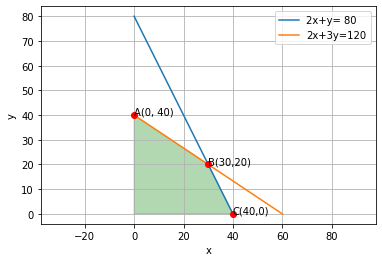
\includegraphics[width=\columnwidth]{solutions/su2021/2/16/Figure 11.png}
\caption{graphical solution}
\label{opt/16/fig: graphical solution}	
\end{figure}
